\chapter{Определение смысловой близости пары ключевых слов} \label{chapt1}
В настоящем разделе подробно описываются алгоритмы определения семантической близости пары ключевых слов. Разработанные модели определения семантической близости является важным результатом деятельност в рамках настоящей диссертации.
Для определения близости вводятся вспомогательные графы, вершинами которых являются ключевые слова, а ребра указывают на некоторые свойства пары ключевых слов.
На основе построенных графов с помощью методов из теории графов вычисляются различные количественные характеристики, необходимые для выявления семантической связи между рассматриваемыми словами.
После этого предлагаются способы применения техник машинного обучения, которые в значительной мере улучшают качество определения смысловой близости между ключевыми словами. 
Также описывается новый алгоритм автоматического формирования обучающей выборки для машинного обучения. Важность данного алгоритма в том, что он избавляет от необходимости ручной разметки данных, которая обычно является трудозатратной работой.
В конце раздела представлены результаты тестовых испытаний программных реализаций алгоритмов, выводы о выполненной работе, а также предлагаются идеи для дальнейшего улучшения качества определения семантической близости наборов ключевых слов.

\section{Графовые алгоритмы выявления семантической информации}
\subsection{Построение графа близости ключевых слов} \label{sect1_1}
Вычисление смысловой близости пары ключевых слов основывается на построении графа ключевых слов. Вершины этого графа соответствуют ключевым словам, а взвешенные ребра отражают факт вхождения слов в один набор. Значение веса ребра между вершинами $i, j$ графа $G$ определяется формулой:
$$ G(i, j) = \sum_{\{T|i\in T, j \in T\}}\frac{1}{|T|}, $$
где суммирование проводится по всем наборам $T$, которые содержат в себе оба слова $i$ и $j$.

Таким образом, если слова часто встречаются в  коротких наборах, то вес соответствующего ребра в графе будет высоким. Эта характеристика является важной для определения семантической близости, но не определяющей: слова не обязаны быть похожими друг на друга по смыслу. Напротив, нередко они служат для того, чтобы более точно описать общую тему документа, к которому относятся, а добавление точного синонима не добавляет информации о тематике документа. 

Следует однако отметить, что в таком виде граф не дает значительного улучшения результата. Это происходит вследствие того, что ребра между непохожими друг на друга вершинами <<зашумляют>> значения формул:   высокое значение формулы начинает больше указывать на уровень употребимости пары слов вместе, чем на семантическую близость между ними. Чтобы избежать подобного эффекта, была разработана более эффективная модель вычисления контекстной близости для пары ключевых слов, описанию которой посвящен следующий далее раздел.


\subsection{Модель определения контекстной близости для пары ключевых слов} %\label{sect1_2}
Важной идеей новой модели вычисления смысловой близости по сравнению с моделью, описанной ранее в главе [???] является следующее наблюдение: уровень похожести слов x и y увеличивается, если существует большое число слов $k$, входящих в одни наборы и с $x$, и с $y$. С учетом этого факта была разработана модель определения контекстной близости, описание которой приводится далее. Согласно проведенным тестовым испытаниям, контекстная близость является более точной аппроксимацией смысловой близости, чем близость, введенная ранее в [???]. Общие слова $k$ в рамках новой модели выступают в роли общего контекста для слов $x$ и $y$. Вычисления контекстной близости для пары вершин производится по графу ключевых слов. При этом высокие частоты вхождений слов $x$ и $y$ в различные наборы негативно влияют на уровень близости: частотные слова склонны иметь больше общих контекстов. Таким образом возникает естественная идея нормировки близости на частоты встречаемости слов, для которых необходимо вычислить уровень близости. 

Кроме того, поскольку слова $x$, $y$ и $k$ могут все входить в один набор, то в таком случае связь слов $x$ и $y$ через слово $k$ будет отражать скорее факт совместной встречаемости $x$ и $y$ в одном наборе, а не контекстную близость этой пары слов. Cовместная встречаемость далеко не всегда влечет сильный уровень семантической близости. Характер этой связи частотности и смысловой схожести во многом зависит от сферы, в которой применяются ключевые слова, и от того, с какой целью пользователи системы эти ключевые используют. Например, ключевые слова для научной публикации редко содержат в себе синонимы, поскольку эти слова используются для того, чтобы дать читателю понять о чем будет статья. Точные синонимы для слов в этом случае не несут никакой дополнительной информации о данной области. Вследствие этого, высокая частота совместной встречаемости не ведет к семантической близости и должна пессимизировать значение формулы контекстной близости. Другим примером являются ключевые слова в социальных сетях. Пользователи используют ключевые слова к документам таким образом, чтобы этот документ было легче найти среди других документов системы. Поэтому, использование синонимов, переводов, транслитерации, различных способов написания ключевых слов помогает в поиске документа. При этом, однако, не добавляет никакой смысловой информации непосредственно к описанию этого документа. Примеры различных наборов ключевых слов из разных областей будут даны в разделе <<Тестовые испытания>>. Исходя из этих соображений, предлагается две представленные далее формулы для вычисления контекстной близости для пары ключевых слов.

Для пары ключевых слов $i$, $j$ контекстная близость определяется по формулам:

\begin{equation}
    \begin{aligned}
       C_{\+}(i, j) = \frac{C(i, j) * \log(1 + m(i,j))}{f(i) + f(j)},\\
       C_{\-}(i, j) = \frac{C(i, j)}{(1 + m(i,j)) * f(i) + f(j)},
    \end{aligned}
\label{eq:test}
\end{equation}
где $C(i,j)$ - контекстная близость между $i$ и $j$ внутри графа, $m(i,j)$- частота совместной встречаемости в наборах пары $i$, $j$, $f(i)$- индивидуальная частота встречаемости слова $i$ в наборах. В программной реализации алгоритмов частоты $f(i)$ и $m(i,j)$ для удобства сохраняются при построении графа ключевых слов в качестве дополнительной информации, соответственно, в вершинах и в ребрах графа.

\subsection{Построение полного контекстного графа ключевых слов}
Вершинами контекстного графа, как и в случае графа, описанного ранее в разделе \ref{sect1_1}, являются ключевые слова. Ребро в таком графе свидетельствует о том, что пара ключевых слов является контекстно близкой. Для того, чтобы определить, соединены ли два ключевых слова ребром, необходимо посчитать контекстную близость по формулам, описанным в предыдущем разделе. В общем случае, для определения всех связей потребовалось бы $O(n^2)$ действий, где $n$- число вершин. Однако с помощью представленного далее алгоритма, это задача может быть решена за $O(nm^2)$ действий, где $m$- максимальное число соседей у вершины в графе ключевых слов.

\begin{enumerate}
    \item Построение графа ключевых слов $G$ по входным наборам ключевых слов $D$
    \item Подсчет частот встречаемости $f(i)$ и $m(p, q)$ для каждого слова $i$ и каждой пары $(p, q)$ по входным наборам из $D$
    \item Инициализация разреженной матрицы $C$ размером $n * n$
    \item Для каждой вершины $i$ графа ключевых слов:
        \begin{enumerate}
            \item Для каждой пары соседей $(p, q)$ вершины $i$:
                \begin{enumerate}
                    \item $C(p, q) \mathrel{{+}{=}} min(G(p,i), G(q,i))$
                \end{enumerate}
        \end{enumerate}
    \item Для каждой ненулевой пары $(i, j)$ матрицы $С$:
        \begin{enumerate}
            \item $C_{\+}(i, j) = \frac{C(i, j) * \log(1 + m(i,j))}{f(i) + f(j)}$
            \item $C_{\-}(i, j) = \frac{C(i, j)}{(1 + m(i,j)) * f(i) + f(j)}$
        \end{enumerate}
\end{enumerate}

\textbf{Утверждение 1.} Расчет весов $C_{+}(i, j)$ и $C_{-}(i, j)$ по построенному графу ключевых слов имеет сложность $O(nm^2)$, где $n$ - число вершин графа ключевых слов, $m$ - максимальное число ребер у вершины в графе ключевых слов.

\textbf{Доказательство.} Поскольку индивидуальные и парные частоты $f(i)$ и $m(i,j)$  уже были рассчитаны при построении графа ключевых слов, их получение имеет сложность $O(1)$.  Остается лишь вычислить сложность подсчета формул $C(p,q)$. Для вычисления требуется пройтись по всемn вершинам графа и для каждой вершины рассмотреть все пары ее соседей. Поскольку у вершины не более $m$ соседей, то обработка одной вершины занимает $O(m^2)$, а всех вершин, соответственно, $O(nm^2)$. Таким образом, и общее время работы алгоритма составляет $O(nm^2)$, что и требовалось доказать.

В целях большей оптимизации времени на построение контекстного графа разумным является ограничения числа рассматриваемых соседей для текущей вершины $i$. Данная оптимизация выполняется следующей модификацией п.4 описанного ранее алгоритма:

\begin{enumerate}
  \setcounter{enumi}{4}
  \item Для каждой вершины $i$ графа ключевых слов:
      \begin{enumerate}
          \item Сортировка соседей вершины $i$ по убыванию весов в ребрах
          \item Выделение множества $N_(i)$- первых $k$ соседей из сортированного в п.4.a списка соседей для вершины $i$
          \item Для каждой пары соседей $(p,q)$ из множества $N_k(i)$ вершины $i$:
              $$ C(p, q) \mathrel{{+}{=}} min(G(p,i), G(q,i)) $$
      \end{enumerate}
\end{enumerate}

В данном случае появляется дополнительный параметр модели $k$ (обычно в диапазоне от 10 до 30), который подбирается исходя из природы коллекции данных, а также по вычислительной производительности машины, на которой запущены расчеты. Отмечается, что предварительная сортировки соседей вершины $i$ по весам ребер позволяет использовать наиболее важных соседей в первую очередь. В результате этого на практике появляется способ значительно уменьшить количество вычислений и при этом построить модель, не уступающую в качестве модели, в которой рассматривается полный набор соседей для вершины. В некоторых случаях удаление менее значимых вершин дает даже прирост в качестве, поскольку зачастую такие вершины являются шумовыми для определения семантической близости.

Построение контекстного графа, в котором для вершины рассматриваются не все ее соседи, имеет вычислительную сложность $O(nk^2+m\log(m))$, что показано в следующем утверждении.

\textbf{Утверждение 2.} Расчет весов $C_{+}(i, j)$ и $C_{-}(i, j)$ по построенному графу ключевых слов для случая ограниченного числа рассматриваемых соседей для текущей вершины имеет сложность $O(nk^2+m\log(m))$, где $n$ - число вершин графа ключевых слов, $k$ - количество рассматриваемых соседей.

\textbf{Доказательство.} Аналогично предыдущему утверждению, за исключением того, что теперь для текущей вершины будет рассмотрено порядка $O(k^2)$ пар соседей. Кроме того появляются дополнительные затраты на сортировку соседей вершины (п.4.а последнего алгоритма), которые занимают $O(m\log(m))$ времени. 

При $k=\sqrt{m}$, например, достигается оценка $O(nm)$ времени работы, что является значительным ускорением работы алгоритма.

Таким образом, данный алгоритм позволяет за время, относительно небольшое по сравнению с наивным перебором всех пар вершин, расчитать контекстный граф, собранный по данным из миллионов наборов ключевых слов, поскольку в среднем каждое слово соединено с небольшим числом других слов. Следует также отметить, что отношение контекстной близости коммутативно, поэтому хранить достаточно только верхний правый угол матрицы $C(p,q)$.

\subsection{Построение усеченного контекстного графа ключевых слов}
Обозначим теперь за $C_{*}(i,j)$ любую из формул $C_{+}(i,j)$ или $C_{-}(i,j)$. Ненулевое значение $C_{*}(i,j)$ означает контекстную связь между ключевыми словами. Несмотря на то, что такие матрицы контекстной близости остаются сильно разреженными, существует огромной число ненулевых связей, что делает затруднительным их дальнейший анализ с технической точки зрения. В дополнении к этому, низкие значения близости могут являться шумом. Такие данные не привносят полезной информации, а только ухудшают качество алгоритмов. По этим причинам возникает практическая необходимость в усечении графа, собранного описанным выше алгоритмом. Под усечением понимается удаление ребер, которые представляют наименее качественные и статистически проверенные связи. 

По результатам экспериментов на коллекциях данных, описанных далее в разделе <<Тестовые испытания>>, была установлена следующая стратегия отбора важных связей для данной вершины $i$:
\begin{enumerate}
    \item \textbf{Для всех $j$ удаляются связи со слишком низким уровнем близости $C_{*}(i,j)$.}

    Этот шаг необходим для того, чтобы удалить <<шумные>> и слабые связи из рассмотрения. Стоит также отметить, что по результатам экспериментов было проверено, что одного этого правила недостаточно для качественного обрезания лишних ребер. Причиной этому является тот факт, что сами значения близости $C(i,j)$ не так важны, как порядок, который они задают на множестве соседей вершины $i$.  Другими словами, данная задачу фильтрации стоит рассматривать как задачу ранжирования соседей вершины $i$ , а не как задачу классификации пар $(i, j)$ на классы полезных и бесполезные ребер.
    \item \textbf{От оставшихся выбирается некоторая доля связей (например, 20\%) с наибольшими значениями $C_{*}(i,j)$ .}

    Это условие видится естественным, потому что слова, которые встречаются со многими другими в одинаковых контекстах, должны иметь больше ребер в графе, чем те слова, которые контекстно близки только с небольшим числом слов.

    \item \textbf{Количество отобранных связей должно находиться в некоторых рамках (например, не менее 3 и не более 10 соседей на вершину).}

    Верхняя граница является преимущественно техническим ограничением: если было взято 20\% от числа всех соседей, но это число по-прежнему достаточно велико, то хранение таких вершин потребует значительных ресурсов. Нижняя граница берется для того, чтобы вершина, для которой имеется мало кандидатов, получила хотя бы их в качестве ребер. С учетом ограничения из п.1. можно ожидать, что эти связи будут достаточно качественными для дальнейшего анализа.
\end{enumerate}

Следует также отметить, что окончательное число соседей для данной вершины $i$ может быть несколько больше, поскольку лишние связи могли породиться одним из соседей вершины в полном графе, это означает, что ребро $(i,j)$ может существовать, потому что оно прошло фильтрацию ребер для вершины $j$, а не для вершины $i$. Далее приведено более формальное описание алгоритма, реализующего введенную выше модель.

\begin{enumerate}
    \item Все значения близости, меньшие порогового  t, приравниваются нулю:

        $$C_{*}(i,j):=0, если C_{*}(i,j) < t. $$
    \item Пусть $rank_j$- порядковый номер соседа $j$ в отстортированном по убыванию значения $C_{*}(i,j)$ списке всех соседей вершины $i$. Тогда, если $rank_j >\max(n_{min},min(n_{max},n * r))$, то связь $(i,j)$ должна быть отфильтрована. Здесь $n_{min},n_{max}$ - минимальное и максимально число ребер для одной вершин в новом графе. $n$- число соседей вершины в полном контекстном графе, $r$- доля ребер, которую необходимо перенести в усеченный граф.
\end{enumerate}

Среди описанных выше параметров только параметр $t$ требует анализа для подбора. Остальные пороговые значения легко могут быть выбраны, исходя из специфики задачи. Подбирать t можно эмпирически или по небольшой размеченной выборке примеров контекстно похожих слов. Отмечается, что tдолжен быть выбран так, чтобы полнота выбранных ребер оставалась достаточно высокой.

Отмечается также, что ребра построенного графа могут быть помечены числами, ввести функцию расстояния между вершинами. Например, такой функцией может служить величина $C_{*}(i,j)$. В рамках рассматриваемого подхода, ребра графа остаются непомеченными, что существенно понижает сложность разработанных моделей.

\subsection{Процедура кластеризации усеченного контекстного графа}
Ребра усеченного контекстного графа, который был введен в предыдущем разделе, в большей мере показывают семантическую близость между парой вершин, чем ребра полного контекстного графа или, тем более, графа ключевых слов. Помимо того, что усеченный граф значительно уменьшает вычислительные затраты, он повышает точность выявленных семантических связей между ключевыми словами, жертвуя при этом полнотой. В этой связи рассмотрение длинных путей в графе становится более оправданным, поскольку семантическая близость между парой вершин лучше сохраняется с увеличением расстояния в графе. Вследствии этого возникает задача кластеризации графа: разделение множества всех вершин на подмножества таким образом, что любая пара вершин из одного множества является парой близких по смыслу ключевых слов. 

За основу кластеризующего алгоритма взят алгоритм Louvain Modularity \cite{louvain_modularity}. В ходе работы алгоритма максимизируется значение функционала модульности: 

$$ Q = \frac{1}{2m}\sum_{i,j}[A_{ij} - \frac{k_i k_j}{2m}]\delta(c_i, c_j) $$

где $\delta$- дельта функция, $A_{ij}$- вес ребра между вершинами $i$ и $j$, $k_i=\sum_j{A_{ij}}, m=\frac{1}{2}\sum_{i,j}A_{ij}$. Как показано авторами \cite{modularity_is_hard}, задача максимизации выписанного выше функционала является NP-сложной, поэтому для её  решения используются аппроксимационный алгоритм, основные шаги которого описаны далее.

\begin{enumerate}
\item Для каждой вершины графа создается свой кластер.
\item Для каждой вершины $i$ и для каждого соседа $j$ вершины $i$:
    \begin{enumerate}
        \item временное добавление вершины $i$ в кластер вершины $j$;
        \item подсчет изменения оптимизируемого функционала $\Delta Q$;
        \item окончательное добавление вершины iв кластер того соседа, на котором достигается максимальное увеличение значения $Q$. Если функционал невозможно увеличить, то добавления не происходит.
    \end{enumerate}
\item Построение нового графа, вершинами которого являются кластера, а веса ребер отражают связи между кластерами. Вес ребра равен сумме весов всех пар ребер, вершины которых лежат в соответствующих кластерах.
\end{enumerate}

Преимущество данного алгоритма в его масштабируемости на графы больших размеров. Качество кластеризации при этом остается на высоком уровне. Отмечается, что количество кластеров не является параметром данного алгоритма. На практике кластера, получающиеся в результате работы программной реализации алгоритма, оказываются слишком большого размера. В некоторые кластера могут попасть тысячи или десятки тысяч слов, очевидно, что не существует такого огромного множества попарно похожих по смыслу слов. Алгоритм является общим графовым алгоритмом и никаким образом не использует информацию о семантической близости. Даже точное решение оптимизационной задачи не гарантирует качественного разбиения вершин графа на подмножества, элементы которого семантически близки друг к другу. Как следствие, необходимы дополнительные действия, связывающие процессы кластеризации графа и определения семантической близости. Далее представлена окончательная версия алгоритма кластеризации контекстного графа, разрешающая отмеченную трудность.

\begin{enumerate}
    \item Заводится очередь для подграфов исходного графа, исходный граф добавляется в нее.
    \item Пока очередь не пуста:
    \begin{enumerate}
        \item кластеризация подграфа из очереди алгоритмом Louvain Modularity;
        \item для каждого полученного в результате кластеризации подграфа-кластера:
            \begin{enumerate}
                \item если размер кластера меньше, чем $k$, то добавить кластер в выходное множество кластеров;
                \item иначе добавить кластер в очередь подграфов.
            \end{enumerate}
    \end{enumerate}
\end{enumerate}

$k$- параметр алгоритма, который выбирается из специфики задачи. Для задачи кластеризации ключевых слов значение параметра $k$ может варьироваться в пределах от 10 до 20.

\subsection{Графовые методы выявление тематических направлений в наборах ключевых слов} %\label{sect1_2}
\subsection{Определение смысловой близости для решения задачи поиска эксперта} \label{expert_search_wordsim}
Постановка и решение задачи поиска эксперта рассматривается в главе \ref{expert_search}. Для ее решения возникает необходимость вычислять похожесть между наборами ключевых слов, характеризующих потенциальных экспертов, с ключевыми словами запроса. Для этого, в свою очередь, разработана базовая процедура для определения близости пары ключевых слов, использующая методы и идеи, которые описаны в настоящей главе.

Вычисление смысловой близости пары ключевых слов также основывается на построении графа ключевых слов, введенного в (???). Вершины этого графа соответствуют ключевым словам, а взвешенные ребра отражают факт вхождения слов в один набор. Другим важным понятием является уровень абстрактности ключевого слова, который описан в главе (???). Под абстрактностью понимается степень общности значения слова. Алгоритм определения степени абстрактности по ключевому слову описан в (???). Для вычисления смысловой близости пары ключевых слов используются следующие далее соображения.

\begin{itemize}
    \item \textbf{Чем ближе друг к другу находятся теги в графе, тем больше они схожи по смыслу.} Другими словами, значение семантической близости обратно пропорционально кратчайшему расстоянию между вершинами в графе. За вес ребра принято число наборов из корпуса, в которые входят оба тега. Если $w(i, j) = |{p \in W_X | i \in p \wedge j \in W_X}|$ ­ вес ребра ($W_X$ - множество всех наборов ключевых слов информационной системы), то за длину ребра принята величина $l_0(i, j) = \frac{1}{1+\log(w(i,j))}$ , где $i$, $j$ ­ смежные вершины. Для случая $i = j$ положим $l_0(i, i) = 0$. Следует отметить, что от функции $l_0(i, j)$ достаточно потребовать лишь обратной зависимости от функции $w(i, j)$ . Тем не менее, описанная выше формула позволяет получить лучший результат, чем, например, наивная формула $\frac{1}{w(i,j)}$.
    \item \textbf{Необходимо использовать только статистически важные связи в графе.} Набор ключевых слов к научной публикации не обязан состоять из похожих по смыслу слов. Например, в одном наборе (<<космический аппарат>>, <<упругие элементы>>, <<процесс отделения>>). Замечается, что ключевые слова <<космический аппарат>> и <<упругие элементы>> не должны обладать сильной семантической связью. Поэтому вводится условие: если количество совместных появлений пары тегов меньше порогового значения $t$ , то такая связь в графе не учитывается. Исключением являются те ребра, удаление которых приводит к увеличению числа компонент связности в графе ключевых слов.
    \item \textbf{Пара слов с более высокими степенями абстрактностей должна обладать меньшим значением семантической близости, чем пара узкоспециальных слов.} В качестве примера рассмотрим следующую ситуацию: пара абстрактных по значению тегов («динамика», «кинематика») и пара более узкоспециальных тегов («прибыль», «доход») могут располагаться на одном расстоянии друг от друга в графе. Однако видно, что пара («прибыль», «доход») явно должна иметь большее значение смысловой близости, потому что оперирует более узкоспециализированными тегами. Исходя из этих соображений можно предположить, что семантическая близость должна зависеть от уровней абстрактностей сравниваемых ключевых слов.
    \item \textbf{Пути графа, проходящие через слова с более высокой степенью абстрактности, должны учитываться с меньшим весом.} Слова, обладающие более широким значением, имеют больше связей с другими словами графа. Это обстоятельство приводит к тому, что существует множество пар узкоспециальных слов, которые явно не являются похожими семантически, однако располагаются при этом близко друг к другу в графе. Обычно такое происходит, если пара слов имеет общую вершину с высокой степенью абстрактности. Например, пара тегов («ленивые вычисления», «оценка максимального правдоподобия») находятся близко друг к другу из­за их связей с тегом «машинное обучение», который является более общим понятием. Можно при этом заметить, что на самом деле слова этой пары далеки друг от друга семантически. По этой причине возникает необходимость «перевзвесить» ребра графа. Обозначим степень абстрактности ключевого слова $x$ за $A(x)$. Величина $A(x)$, исходя из введенного в главе (???) определения, не превышает  1. Положим теперь длину ребра равной $l(i, j) = \exp(\frac{l_0(i, j)}{\log(A(i))\log(A(j))})$. Таким образом, чем выше степени абстрактности вершин, инцидентных данному ребру, тем больше длина этого ребра. Длина кратчайшего пути между вершинами $v_x, v_y$ принята за $L(v_x,v_y)$ . Экспонента в формуле делает значение $l(i, j)$ не меньшим, чем 1.
    \item \textbf{Чем больше различных связей (путей) между вершинами в графе, тем больше уровень семантической близости.} При этом дополнительную информацию дают веса ребер. Это следует из того, что если два тега связаны тяжелым ребром или путь между ребрами имеет большой вес, то такие теги будут более близки по смыслу, чем аналогичная пара с легкими ребрами. В этой связи возникает необходимость решения задачи определения максимального потока между двумя вершинами графа. В классической постановке требуется для пары вершин, называемых источником и стоком, транспортной сети найти такой поток из источника в сток, что его величина будет максимальна. На граф тегов эта задача переносится очевидным образом, если ребра принять за двунаправленные, а за пропускную способность ребра ­ его вес. При этом пропускная способность считается отдельно для каждого из направлений. Пусть максимальный поток между вершинами $v_x, v_y$ равен $MaxFlow(v_x, v_y)$. Максимальной вместимостью вершины назовем сумму весов ребер, входящих в нее. Обозначим максимальную вместимость вершины $i$ за $C(i)$. Тогда за $F(v_x,v_y)$ примем величину, равную $\frac{MaxFlow(v_x,v_y)}{min(C(v_x), C(v_y))}$. В этом случае $F(v_x,v_y)$ показывает, насколько использована пропускная способность канала между вершинами. Максимум, равный единице, достигается, если пропускная способность использована полностью. В частности, $F(vx,vx) = 1$.
\end{itemize}

Учитывая перечисленные выше cоображения, формула близости между парой ключевых слов $x$ и $y$ вводится следующим образом:

$$ WordSim_{expert}(x, y) = \frac{F(v_x, v_y)}{L(v_x, v_y)}, $$

где $v_x$ и $v_y$ - пара вершин в графе ключевых слов, соответствующая ключевым словам $x$ и $y$.


\subsection{Тестовые испытания} \label{test_sect}
В настоящем разделе описаны результаты тестовых испытаний программных реализаций описанных ранее алгоритмов. В качестве тестовых данных были использованы корпусы ключевых слов для научных публикаций, собранных из сети Интернет. Использовалась также информация из социальной сети Вконтакте, а именно - были выкачаны посты (публичные сообщения из групп и страниц пользователей), часть из которых помечены хэштегами. В процессе сбора данных проводился парсинг текстовых данных на предмет наличия в них наборов ключевых слов. Точное решение этой задачи не является предметом исследования данной работы (???), поэтому для парсинга данных были использованы наивные подходы, которые, тем не менее, позволяют собрать корпус достаточного размера и качества  для проведения дальнейшего анализа.
В конечном итоге собрано два объемных набора данных:
\begin{itemize}
    \item 329.000 наборов для русского языка;
    \item 3.069.000 наборов хэштегов из сети Вконтакте.
\end{itemize}
Далее приведены примеры наборов ключевых слов из обоих источников. Наборы ключевых слов научных публикаций:

    \textbf{[топонимический концепт, языковое сознание, когнитивная база, прецедентность, апеллятивация]}\

    \textbf{[вариабельность сердечного ритма, гребля на каноэ, вегетативный тонус]}\
    
    \textbf{[архитектуры, деформации, геологическая среда, сфера взаимодействия]}

Наборы хэштегов из социальной сети:

    \textbf{[electro\_pop, dance, fresh, music, new\_zealand]}\

    \textbf{[vitaminhealth, oxygenwater, waterhealth]}\

    \textbf{[bodyfan, питание, bodyfanпитание, bodyfanmotivation, motivation, bodybuilding, фитнес, gym, спорт, мотивация, зож]}

\subsubsection{Определение семантической близости с использованием графов ключевых слов}
Программные реализации описанных в предыдущих главах алгоритмов были применены к собранным данным. Далее на рисунке \ref{img:sim_1} представлены ближайшие соседи для слов <<федерация>> и <<регионы>> в графе ключевых слов.

\begin{figure}[ht]
  \begin{minipage}[ht]{0.49\linewidth}\centering
    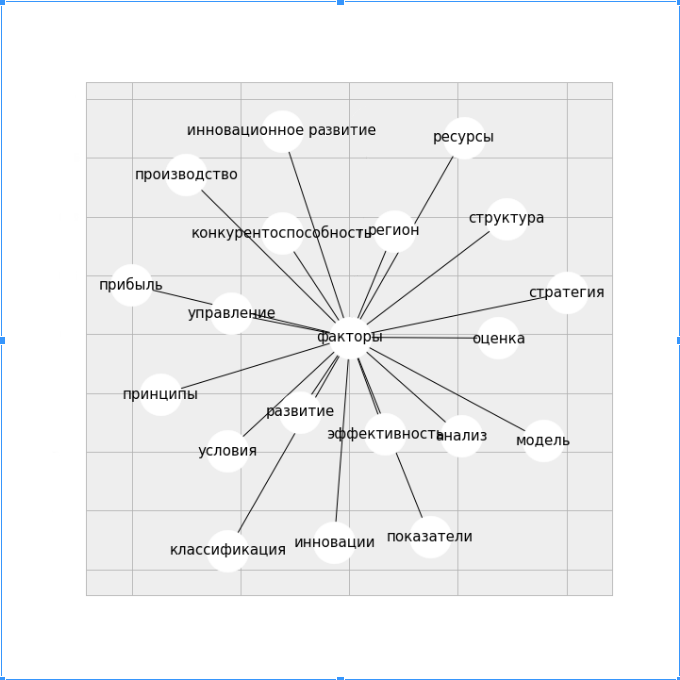
\includegraphics[width=1.0\linewidth]{Dissertation/pics/factory_sim} \\ а)
    \caption{Соседи вершины <<факторы>> в графе ключевых слов}
  \end{minipage}
  \hfill
  \begin{minipage}[ht]{0.49\linewidth}\centering
    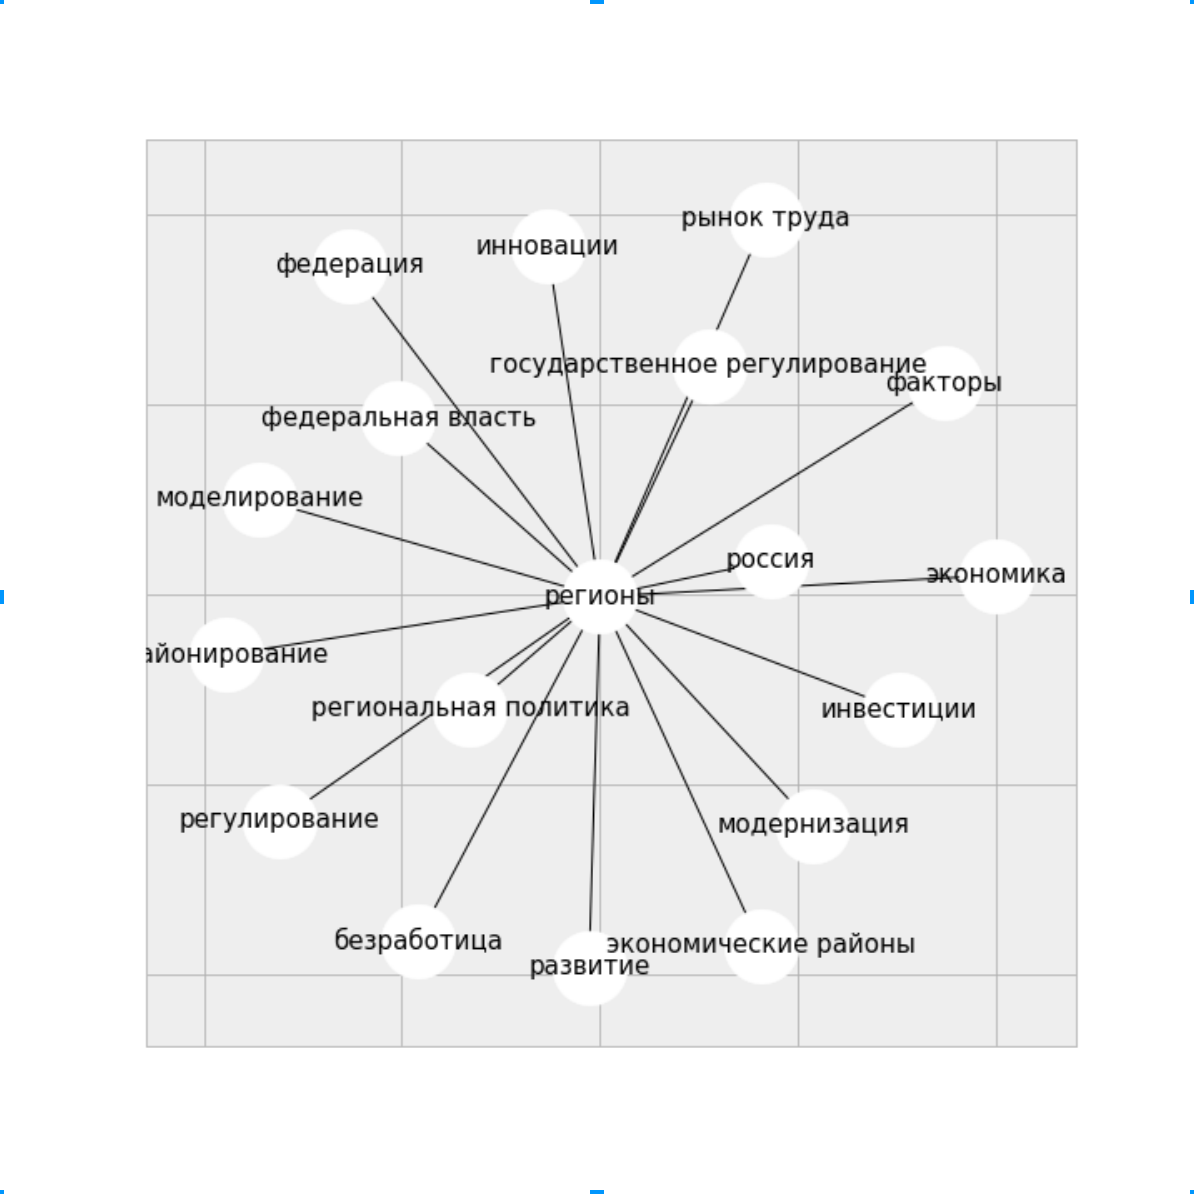
\includegraphics[width=1.0\linewidth]{Dissertation/pics/regiony_sim} \\ б)
    \caption{Соседи вершины <<регионы>> в графе ключевых слов}
  \end{minipage}
  \label{img:sim_1}
\end{figure}

На рисунках выше видно, что графа ключевых слов не хватает для определения семантической близости пары слов: видно, что существуют связи такие, как <<факторы-модель>>, <<регионы-экономика>>, которые не обладают явной смысловой связью. Применение методов построения усеченного контекстного графа дает значительное улучшение качества классификации пар ключевых слов на семантически близкие и далекие. Далее указаны примеры найденных пар ключевых слов, близких по смыслу:

\textbf{β-адреноблокаторы   -   бета-адреноблокаторы}

\textbf{новые виды   -   новый вид}

\textbf{орви   -   острые респираторные вирусные инфекции}

\textbf{текущий уровень информационной безопасности   - политика информационной безопасности}

\textbf{умения   -   навыки}

\textbf{образное мышление   -   художественный вкус}

\textbf{хехцир   -   khekhtsyr}

\textbf{рынок банковских услуг   -   банковский рынок}

\textbf{тромболизис   -   тромболитическая терапия}

\textbf{параллельные алгоритмы   -   параллельное программирование}

\textbf{феминность   -   фемининность}

\textbf{полином  -  многочлен}

\textbf{корень  -   корни}

\textbf{primerun  -  примерун}

\textbf{fvk  -  fotovideoclub}

\textbf{еврореволюция  -   єврореволюція}

\textbf{silk\_plaster    -  шелковая\_штукатурка}

Интересным фактом является определение похожих слов для заданного многозначного слова. В то время как граф в графе ключевых слов соседями для слова <<орган>> являются слова <<государство>>, <<сибирь>>, <<контроль>>, <<циркуляция>>, <<управление>>, в контекстном графе ближайшими являются слова <<музыковедение>>, <<организм>>, <<отклонение>>, <<делегирование полномочий>>, <<объект контроля>>. Таким образом восстанавливается не только значение слова, связанное с юриспруденцией, но и близкие слова для значения из области музыки (<<музыковедение>>) и биологии (<<организм>>).

На рисунке \ref{img:sim_2} изображены несколько ближайших контекстно близких слов для слова <<студенты>> (отмечается, что полное множество соседей вершины слишком велико, чтобы его изобразить):

\begin{figure}[ht]
  \begin{minipage}[ht]{1.0\linewidth}\centering
    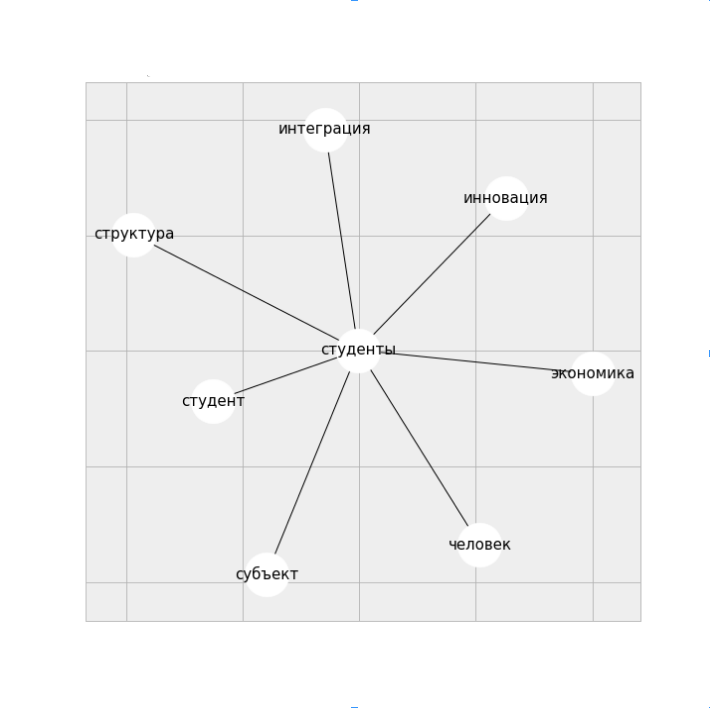
\includegraphics[width=1.0\linewidth]{Dissertation/pics/students_sim}
    \caption{наиболее близкие слова для слова <<студенты>> в контекстном графе}
  \end{minipage}
  \label{img:sim_2}
\end{figure}


\subsubsection{Построение кластеров семантически похожих ключевых слов}

Описанный ранее алгоритм кластеризации контекстного графа позволяет удалять недостаточно надежные связи между словами, полученные с помощью алгоритма определения близости по контекстному графу, и, наоборот, добавлять новые ребра между семантически похожими парами слов. 

Кластер для слова <<студенты>> изображен на рисунке \ref{img:clust_1}

\begin{figure}[ht]
  \begin{minipage}[ht]{1.0\linewidth}\centering
    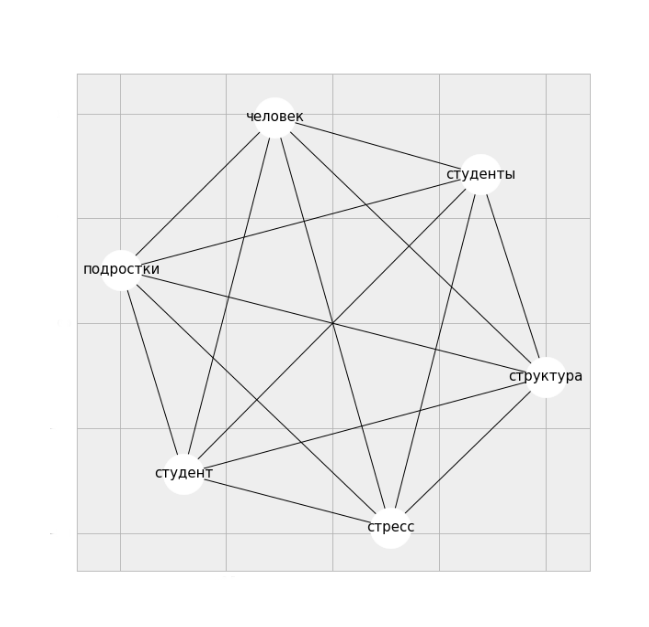
\includegraphics[width=1.0\linewidth]{Dissertation/pics/students_cluster}
    \caption{кластер, содержащий слово <<студенты>>}
  \end{minipage}
  \label{img:clust_1}
\end{figure}

Можно заметить, как в результате кластеризации были разорваны связи <<студенты-экономика>>,  <<студенты-инновации>>, вместо которых на первый план вышли связи <<студенты-подростки>>. Отмечается также, что выбранный метод кластеризации графа может допускать ошибки. Например, в случае с парой <<студенты-структура>>, которая была как в усеченном контекстном графе, так и в кластере слова студент.

Для интегральной проверки качества была выбрана следующая методика.

\begin{enumerate}
    \item Набирается набор пар ключевых слов, для которых можно  определить их высокий уровень семантической близости посредством детерминированного алгоритма (положительные примеры). Пара слов определяется близкой по смыслу, если выполняется хотя бы одно из условий:
    \begin{enumerate} 
        \item одно ключевое слово является аббревиатурой для другого;
        \item расстояния Левенштейна между парой невелико.
    \end{enumerate}
    \item К зафиксированным семантически похожим парам слов добавляются отрицательные примеры, т.е. пары слов, которые не являются близкими по смыслу. Для этого проводятся следующие шаги:
        \begin{enumerate}
            \item если пара слов $(a,b)$ определена на первом шаге как пара похожих слов, то для слова aберется $k$ случайных соседей $c_1, c_2, \dots,c_k$ из графа ключевых слов на расстоянии, не превышающем 2; 
            \item все пары $(a,c_i)$ определяются как отрицательные примеры.
        \end{enumerate}
    \item Положительные и отрицательные примеры составляют тестовую выборку. После чего для всех пар тестовой выборки вычисляется близость, по формулам описанным выше, а также подбирается порог, по которому в зависимости от вычисленного значения близости пара относится либо к классу семантически близких пар, либо к классу семантически далеких.
    \item По оценкам классификатора и тестовой выборке считается F-мера, которая и является показателем качества алгоритма.
\end{enumerate}

В результате тестирования программной реализации алгоритма получено высокое  по отношению к реализованным в [???] алгоритмам значение F-меры - 0.82. Проведение аналогичного теста для алгоритма определения близости лишь с помощью анализа частотности встречаемости пары слов дает результат 0.67, таким образом, методы, описанные в данной работе существенно улучшают качество определения семантической похожести. Отмечается, что выбранный способ тестирования имеет очевидный недостаток: среди положительных примеров очень редко встречаются пары смысловых синонимов, напротив, они могут попадать в пары отрицательных примеров. Тем не менее, по экспертной оценке увеличение качества на описанной ранее тестовой выборке влечет улучшение качества классификации и более сложных пар ключевых слов, таких как  пар <<синоним>>-<<синоним>> или <<слово>>-<<перевод слова на другой язык>>.

\subsubsection{Апробация автоматического тематического классификатора}
...
\subsection{Выводы}
По результатам исследований, результаты которых представлены в разделе \ref{test_sect}, построены модели определения близости по корпусу наборов ключевых слов, опирающиеся на методы из теории графов. Для данных моделей представлены алгоритмы и созданы программные реализации этих алгоритмов. Реализации были протестированы на двух коллекциях наборов ключевых слов и был получен относительно высокий уровень качества результатов. Кроме того, была разработана модель кластеризации ключевых слов, опирающаяся на введенные графовые модели представления коллекций ключевых слов и на построенную по этим графам меру схожести для пары слов. Программная реализация процедуры кластеризации также протестирована, для нее был получен высокий уровень качества определения кластеров схожих ключевых слов.
\textbf{??? добавить текст про тематический классификатор}
Недостатком работы может являться большое число параметров, которое необходимо настроить. В качестве дальнейшего направления в изучении данной области автор настоящей дисертации считает целесообразным применения техник машинного обучения для построения меры близости между ключевыми словами. Такой шаг поможет избавиться от значительной части параметров описанных в предыдущих главах моделей, предоставив возможность настройки этих параметров в автоматическом режиме.

\section{Использование техник машинного обучения для улучшения модели близости слов}
...
\subsection{Методы формирования обучающей выборки}
...
\subsubsection{Ручные методы}
...
\subsubsection{Автоматические методы}
...
\subsection{Признаковое описание модели машинного обучения}
...
\subsection{Описание и настройка модели машинного обучения}
...

\subsection{Тестовые испытания}
...
\section{Построение тезауруса ключевых слов по коллекции наборов}
...
\subsection{Алгоритм построения}
...
\subsection{Тестовые испытания}
...
\section{Методы кластеризации ключевых слов по графам ключевых слов}
...
\section{Выводы}
